\section{Cook's theorem and the complexity of variants of SAT.}

\subsection{Disposition}

\begin{enumerate}
 \item \textbf{Def. P, NP, NP-hard \& NPC}
    \subitem  Tegn!
 \item \textbf{Def. Reduktioner}
    \subitem  Proposition 3: Transitivitet (v. bevis)
    \subitem  Proposition 4: Nedadgående lukkethed af P
 \item \textbf{Lemma 7:} \textit{Hvis $L_1 \in$ NP-hard og $L_1 \leq L_2$, så er $L_2 \in$ NP-hard}
    \subitem  Bevis
 \item \textbf{Def. CNF \& Boolean Circuits}
 \item \textbf{Cook's Theorem}
    \subitem Def. SAT
    \subitem Def. CIRCUIT SAT
 \item \textbf{Theorem 11:} \textit{CIRCUIT SAT $\in$ NPC}
    \subitem Bevis.
 \item \textbf{Proposition 12:} \textit{CIRCUIT SAT $\leq$ SAT}
    \subitem Bevis.
 \item \textbf{Proposition 9.2:} \textit{3SAT $\in$ NPC}
    \subitem Vis SAT $\leq$ 3SAT.
\end{enumerate}

\subsection{Emne detaljer}

Følgende afsnit indeholder detaljer om hvert punkt i dispositionen ovenfor (og muligvis flere ting også).


\subsubsection{Def. P, NP, NP-hard \& NPC}

Lad os starte med lige at kigge på de kompleksitetsklasser vi har arbejdet med her i kurset.
\begin{center}
 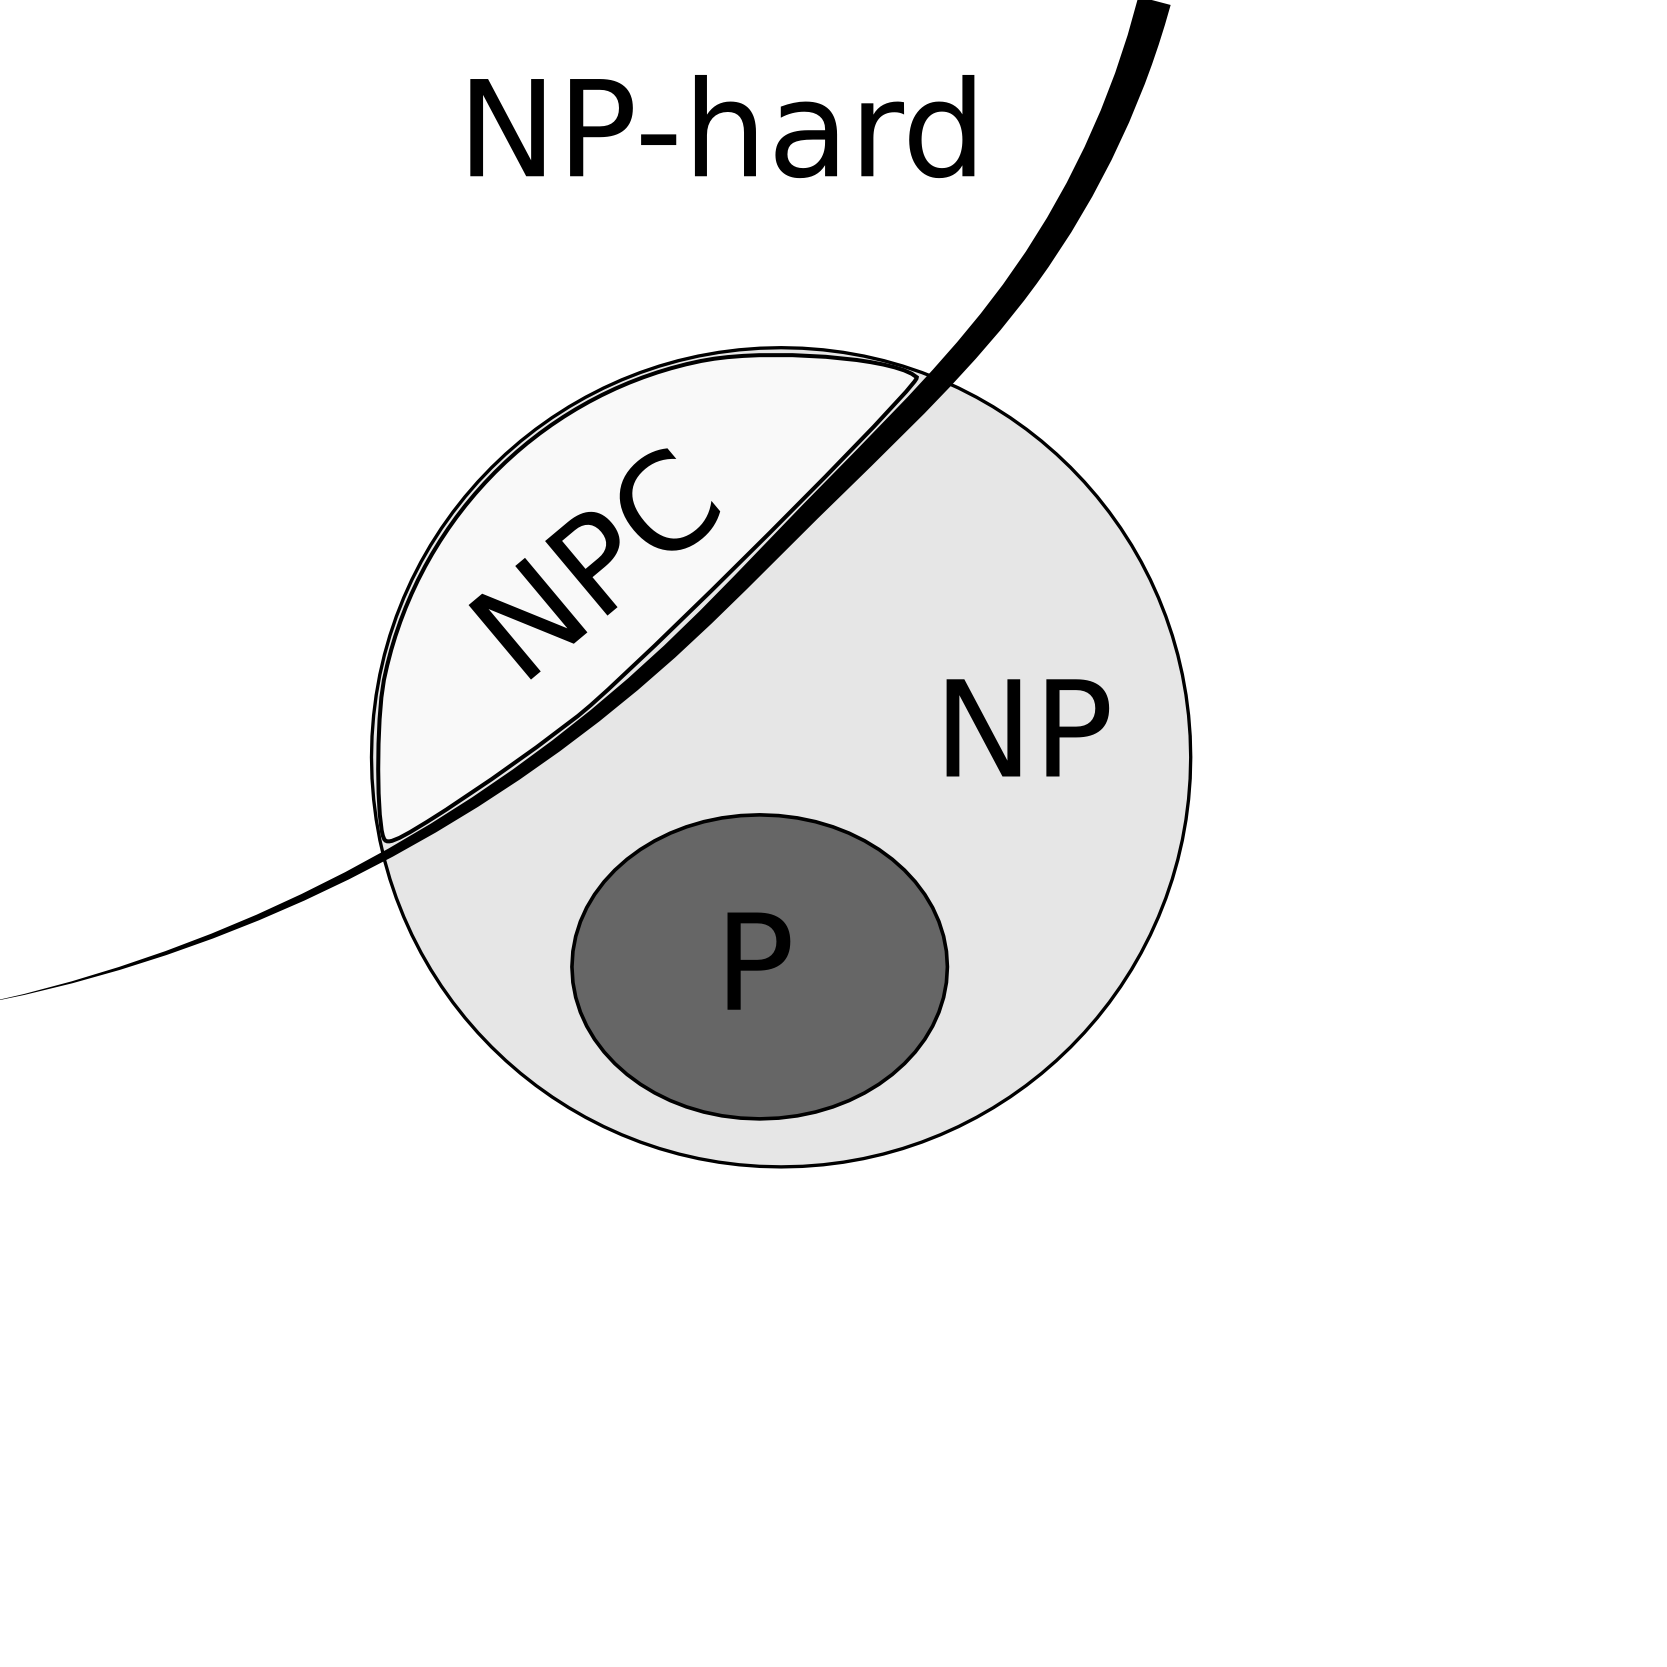
\includegraphics[bb=0 0 400 400,scale=0.3]{./PNPNPC.png}
 % PNPNPC.png: 1667x1667 pixel, 300dpi, 14.11x14.11 cm, bb=0 0 400 400
\end{center}


\paragraph{P}
~\\
~\\
Kompleksitetsklassen $P$ er formelt defineret således:
\begin{align*}
 P = \left\lbrace L \subseteq \left\lbrace 0,1 \right\rbrace^* | \exists \text{ TM } M_L \text{ der afgører L i polynomiel tid } \right\rbrace
\end{align*}
Altså klassen af beslutningsproblemer der kan blive bestemt af en deterministisk Turing Maskine hvor antallet af ``steps'' maskinen udfører for et givent $x$ maksimalt er $\rho(x)$ for et givent polynomiel $\rho$.\\
 
Intuivit ser vi kompleksitetsklassen $P$ som en klasse for problemer for hvilket vi kender en effektiv løsning. Altså ethvert problem med worst-case kørselstid på formen $O(n^k)$ for et givent $k$.

At worst-case kørseltid på et problem er polynomiel betyder dog ikke reelt at det er et nemt problem (modsat hvad Cobham's Thesis påstår). I hele den analyse ignorerer vi fuldkommen konstanter, samt forventet kørselstid som I mange tilfælde kan få ``sværere'' problemer til at køre bedre end ``nemme'' problemer i $P$.


\paragraph{NP}
~\\
~\\
Kompleksitetsklassen $NP$ er lidt mere kluntet formelt defineret, så vi starter lige med intuitionen først.

Intuitivt kan $NP$ ses som klassen af beslutningsproblemer for hvilket ``yes'' instanserne kan verificeres i polynomiel tid på en deterministisk Turing Maskine. Altså er det komplekse problemer med eksponentiel løbetid, men hvor løsningen til et sådant problem nemt kan verificeres til at være korrekt.\\
~\\
Kompleksitetsklassen $NP$ er formelt defineret således:
\begin{align*}
 NP = \left\lbrace L \subseteq \left\lbrace 0,1 \right\rbrace^* | \exists \rho \in Z[x], L' \in P, \forall x \in \left\lbrace 0,1 \right\rbrace^* : ( x \in L \Leftrightarrow \exists y \in \left\lbrace 0,1 \right\rbrace^* : |y| \leq \rho(|x|) \wedge \left\langle x,y \right\rangle \in L') \right\rbrace
\end{align*}
Definitionen skal forståes således: Vi har et sprog $L' \in P$, samt et polynomiel $\rho$. Vi tænker så nu på et sæt af binære strenge af længde maksimalt $\rho(|x|)$, hvor disse representerer mulige løsninger til probleminstansen $x$. Med denne fortolkning bliver $\left\langle x,y \right\rangle \in L'$ så måden hvorpå vi tester om en given løsning $y$ virkelig er en korrekt løsning. 

Denne form for søgningsproblem kaldes ofte for et simpelt søgningsproblem, da den kan verificeres i polynomiel tid, men ikke løses deri (antaget $P \neq NP$).\\

For at løse et givent NP problem kunne vi så løbe igennem alle mulige løsninger for $y$, som sammenlagt ville være $2^{\rho(|x|)+1}-1$, og for hver af dem tjekke $\left\langle x,y \right\rangle \in L'$. Det ønsker vi dog ikke, da det ville tage eksponentiel tid. I stedet forsøger man ofte at finde snedige måder at lave speed-ups og/eller lave approximationsalgoritmer af forskellige art.

Og i visse tilfælde er man også heldig at finde en algoritme i $P$ for et $NP$ problem, hvorved man har vist at problemet i virkeligheden ligger i $P$ som jo er et subset af $NP$.

\paragraph{NP-hard}
~\\
~\\
Et sprog defineres som NP-hard såfremt der gælder:

\begin{align*}
 \forall L' \in NP: L' \leq L
\end{align*}

Altså gælder der, at ethvert sprog $L'$ i NP kan reduceres til $L$. Intuitionen er her, at algoritmen til at løse NP-hard problemet er så stærk (eller generel) at den kan bruges til at løse ethvert andet problem i NP. Man siger desuden, at et NP-hard problem således er mindre sandsynlig end noget andet sprog i NP, til at være i P.\\

Navnet kan dog være lidt forvirrende, da et NP-hard problem faktisk ikke behøver være i NP og hvis de er, så kaldes de faktisk ikke engang bare NP-hard længere.

\paragraph{NPC}
~\\
~\\
NP-Complete (NPC) er den særlige klasse af problemer der både er NP-hard og befinder sig i NP. Formelt defineret således: 

\begin{align*}
 NPC = \left\lbrace L \in \left\lbrace 0,1 \right\rbrace^* | L \in NP \wedge (\forall L' \in NP: L' \leq L) \right\rbrace
\end{align*}

NPC problemer er særligt interessante, da vi kan bruge dem til at bevise et givent problem er NP-Complete, således vi ikke spilder tid på forsøg med at finde en algoritme i $P$ for problemet (antaget $P\neq NP$). Dette gør vi vha. noget vi kalder reduktioner.

\subsubsection{Def. Reduktioner}

Det bringer os så til en grundlæggende metode i computationel kompleksitetsteori, nemlig reduktioner. Først og fremmest den formelle definition.

Givet to sprog $L_1$ og $L_2$, en polynomiel reduktion $r$ af $L_1$ til $L_2$ er en polynomial time computable map for hvilken der gælder:

\begin{align*}
 \forall x : x \in L_1 \text{ hviss. } r(x) \in L_2
\end{align*}

Dette skrives som $L_1 \leq L_2$, hvor man læser det som at $L_1$ reduceres til $L_2$. Intuitivt betyder reduktion blot, at vi kan oversætte enhver given instans af $L_1$ til en anden instans af $L_2$. Vi siger desuden, at $L_2$ er et mere generelt sprog end $L_1$ og kan derfor ses, som værende mere sandsynlig til ikke at være i $P$.


Herudover har  reduktioner desuden to nyttige egenskaber vi skal bruge senere.

\paragraph{Proposition 3: Hvis $L_1 \leq L_2$ og $L_2 \leq L_3$, så gælder der $L_1 \leq L_3$}
~\\
~\\
Denne proposition underbygger, at reduktioner er transitive. Vi beviser den således:

\begin{proof}
 Vi har polynomial time computable maps $r_1()$ og $r_2()$, hvor følgende ting gælder:

\begin{itemize}
 \item For ethvert $x$ gælder der, at $x \in L_1$ hvis og kun hvis $r_1(x) \in L_2$.
 \item For ethvert $y$ gælder der, at $y \in L_2$ hvis og kun hvis $r_2(y) \in L_3$.
\end{itemize}

Således har vi for alle $x$, at $x \in L_1$ hvis og kun hvis $r_2(r_1(x)) \in L_3$. Og siden vi blot har brugt to polynomial time computable maps efter hinanden (hvormed det hele kan ses som en polynomial time computable map), så har vi $L_1 \leq L_3$.
\end{proof}

\paragraph{Proposition 4: Hvis $L_1 \leq L_2$ og $L_2 \in P$, så er $L_1 \in P$.}

Proposition 4 siger intuitivt, at $P$ er lukket nedad under reduktion. 

\subsubsection{Lemma 7}

For at kunne bevise et givent sprog er NP-hard, så bruger vi polynomielle reduktioner fra kendte NP-hard problemer, fremfor at forsøge et direkte bevis. For at kunne lave disse reduktioner, så har vi brug for følgende lemma.\\
~\\
\textbf{Lemma 7:} Hvis $L_1$ er NP-hard og $L_1 \leq L_2$ så er $L_2$ også NP-hard.

\begin{proof}
 Siden $L_1$ er NP-hard, så ved vi alle sprog $L$ i NP kan reduceres til det ($\forall L \in NP: L \leq L_1$). Så når $L_1 \leq L_2$, så kan vi bruge transitivitetsreglen (Proposition 3) og konkludere at ethvert sprog $L$ reducerer til $L_2$ ($\forall L \in NP: L \leq L_1 \leq L_2$), hvormed $L_2$ altså er NP-hard.
\end{proof}

\subsubsection{CNF \& Boolean Circuits}

Nu har vi som sådan alle grundstenene på plads til at kunne bevise forskellige problemer er NP-Complete. Men for at fuldføre de specifikke beviser vi gerne vil her, så skal vi lige bruge 2 ting mere: Nemlig CNF formler og Boolean Circuits, eller oversat: boolske kredsløb.\\

\paragraph{CNF}
~\\
~\\
Conjunctive Normal Form, eller CNF, er en særlig måde hvorpå man kan skrive boolske formler. Reglerne for CNF er følgende:
\begin{enumerate}
 \item De eneste mulige funktioner er AND, OR og NOT
 \item Ingen klausuler må indeholde AND
 \item NOT må kun bruges foran konstanter, ikke klausuler
\end{enumerate}
~\\
Således får man, at følgende er skrevet på CNF form:
\begin{align*}
 (A \vee B) \wedge (\neg B \vee C \vee \neg D) \wedge (D \vee \neg E)
\end{align*}
Hvorimod ingen af følgende er f.eks.:
\begin{align*}
 &(A \vee B) \wedge \neg(\neg B \vee C \vee \neg D) \wedge (D \vee \neg E) \\
 &(A \vee B) \wedge (\neg B \wedge C \wedge \neg D) \wedge (D \vee \neg E) \\
 &(A \vee B) \vee \neg(\neg B \vee C \vee \neg D) \vee (D \vee \neg E)
\end{align*}

\paragraph{Boolske kredsløb}
~\\
~\\
Et boolsk kredsløb er en rettet, acyklisk graf $G=(V,E)$ med $n$ input gates, $m$ output gates og hvor knuderne i $V$ ligeledes er gates. Hver gate har desuden en label som indikerer hvilken type gate vi har at gøre med. Disse labels tages så fra følgende samling af funktiontyper:
\begin{align*}
 \left\lbrace AND, OR, NOT, COPY \right\rbrace
\end{align*}
... eller fra sættet af konstante symboler: 
\begin{align*}
 \left\lbrace 0,1 \right\rbrace
\end{align*}
... eller fra et sæt af variabel symboler:
\begin{align*}
 \left\lbrace X_1, X_2, \hdots, X_n \right\rbrace
\end{align*}
Der må desuden maksimalt være en gate med et givent variabel symbol $X_j$, da disse er inputgates. Tilsvarende er der som sagt $m$ output gates $o_1,o_2,\hdots,o_m$.

Alle kanter i grafen $G$ kaldes for wires. Så hvis der er en wire fra gate $u$ til gate $v$, så siger vi $u$ fungerer som input til $v$.\\
~\\
Vi kan nu bruge disse boolske kredsløb til at beregne en boolsk funktion $f: \left\lbrace 0,1 \right\rbrace^n \rightarrow \left\lbrace 0,1 \right\rbrace^m$, ved at evaluere kredsløbet på en given inputvektor $x \in \left\lbrace 0,1 \right\rbrace^n$ hvor værdierne heri tildeles de enkelte inputgates.\\

\subsubsection{Lemma 8}

Vi har følgende lemma der viser, at vi vha. et boolsk kredsløb kan beregne enhver boolsk funktion. Lemmaet bruges uden bevis.\\
~\\
\textbf{Lemma 8:} For enhver boolsk funktion $f: \left\lbrace 0,1 \right\rbrace^n \rightarrow \left\lbrace 0,1 \right\rbrace^m$ findes der et kredsløb $C$, for hvilken der gælder: $\forall x \in \left\lbrace 0,1 \right\rbrace^n: C(x) = f(x)$. 

\subsubsection{Lemma 9}

Vi har desuden følgende nødvendige lemma der kobler tidsfaktoren i en Turing maskine til størrelsen af et boolsk kredsløb. Lemmaet fremvises endnu engang uden bevis.\\
~\\
\textbf{Lemma 9:} Vi har en given Turing maskine $M$ kørende i tid maksimalt $\rho(n) \geq n$ på input af længnde $n$, hvor $\rho$ er et polynomie.

Så gælder der, givet en fastsat inputstørrelse $n$, at vi har et kredsløb $C_n$ med størrelsen maksimalt $O(\rho(n)^2)$, således at der gælder for alle $x \in \left\lbrace 0,1 \right\rbrace^n: C_n(x) = 1$ hvis og kun hvis $M$ accepterer $x$.

Desuden er funktionen der mapper $1^n$ til en beskrivelse af $C_n$ polynomielt tidsberegnelig.\\
~\\
At ovenstående gælder er dog på ingen måde ulogisk, da en reel computer alligevel består af boolske kredsløb når vi går på tilstrækkelig lav-niveau. Vi kan altså bruge boolske kredsløb både som kombinatoriske objekter og som beregningsenheder. \\
~\\
\textbf{TODO: } Til eksamen i Q4 2010 blev mange spurgt om bevis for ovenstående lemma. Det kunne måske være smart at øve det.

\subsubsection{Cook's Theorem}

Det bringer os så videre til hovedemnet her, nemlig Cook's Theorem. Vi vil jo gerne kunne vise at diverse problemer er NP-Complete, men for at gøre det vha. reduktioner, så skal vi først have et NP-Complete problem at starte ud fra.

Takket være Stephen Cook fik vi i 1972 netop lige det, da han viste at SATISFIABILITY PROBLEMET, forkortet SAT, var NP-hard. Herefter kunne mange andre så bruge SAT til at reducere til andre problemer, for at vise at disse nye problemer var NP-hard. Cook beviste oprindeligt SAT ved at vise alle problemer i NP reducerede til SAT, hvilket er en noget kompliceret affære. Derfor vil vi i stedet vise et relateret problem CIRCUIT SAT er NP-hard og så reducerer dette til SAT.

Lad os derfor først og fremmest se på definitionerne på disse to problemer og derefter gå i gang med de egentlige to dele af beviset:

\begin{itemize}
 \item CIRCUIT SAT $\in$ NPC (Theorem 11)
 \item CIRCUIT SAT $\leq$ SAT (Proposition 12)
\end{itemize}

\paragraph{Def. SAT}
~\\
~\\
Givet en CNF formel, er der en tildeling af sandt/falsk til variablerne således hele udtrykket evaluerer til sandt?\\
~\\
\textit{Note: SAT $\in$ NP, siden vi kan evaluere en given boolsk funktion på en bitvektor i polynomiel tid og verificere hvorvidt vi har en tilfredsstillende tildeling. At finde en tilfredsstillende tildeling direkte kræver dog exhaustive search i eksponentielt mange muligheder.}

\paragraph{Def. CIRCUIT SAT}
~\\
~\\
Givet et boolsk kredsløb $C$, er der en inputvektor $x \in \left\lbrace 0,1 \right\rbrace^n$ således at $C(x) = 1$?
~\\
\textit{Note: CIRCUIT SAT $\in$ NP, siden vi kan evaluere et givent kredsløb på en inputvektor i polynomiel tid og verificere hvorvidt vi har en tilfredsstillende tildeling. At finde en tilfredsstillende tildeling direkte kræver derimod exhaustive search eksponentielt mange muligheder.}

\subsubsection{Theorem 11}

Som første skridt mod at bevise SAT er NPC, skal vi først vise CIRCUIT SAT er det. Det gør vi så i følgende theorem.\\
~\\
\textbf{Theorem 11:} CIRCUIT SAT $\in$ NPC

\begin{proof}
 Vi ved allerede at CIRCUIT SAT er i NP. Vi skal derfor bare bevise at CIRCUIT SAT er NP-hard, altså at alle sprog i NP reducerer til det.

Så lad $L$ være et sprog i NP, så må vi nu vise at der er en polynomieltids reduktion $r$ således følgende gælder:
\begin{align*}
 \forall x: x \in L \Leftrightarrow r(x) \in \text{ CIRCUIT SAT }
\end{align*}
Siden $L \in NP$, så ved vi ud fra definitionen, at der er et sprog $L' \in P$ og et polynomie $\rho$ således vi har:
\begin{align*}
 \forall x : x \in L \Leftrightarrow (\exists y \in \left\lbrace 0,1 \right\rbrace^* : |y| \leq \rho(|x|) \wedge \left\langle x,y \right\rangle \in L')
\end{align*}
Nu kan vi så definerer vores reduktion $r$. Reduktionen skal afbildle instanser af $L$ over i instanser af $CIRCUIT SAT$, således at givet et input $x$, så er værdien af $r(x)$ en beskrivelse af et kredsløb $C$. Denne $C$ skal så indeholde $\rho(|x|)$ delkredsløb kombinereret vha. $\rho(|x|)-1$ OR-gates således:
\begin{align*}
 C = D_0 \vee D_1 \vee \hdots \vee D_{\rho(|x|)}
\end{align*}
Hvert af disse delkredsløb $D_i$ skal så tage $i$ inputs og skal returnere $1$ på et givent input $y \in \left\lbrace 0,1 \right\rbrace^i$ hvis og kun hvis $\left\langle x,y \right\rangle \in L'$ - altså kun hvis $y$ er en løsning for den givne instans.\\

Hvis vi kan opnå dette, så har vi tydeligt at $x \in L \Leftrightarrow C \in \text{ CIRCUIT SAT }$.\\
~\\
Lad os så sige vi har en Turing maskine $M$ der afgører $L'$ i polynomiel tid. Ud fra Lemma 9 ved vi, at vi givet en fast inputlængde $n$ har en algoritme der kan outputte et kredsløb $C_n$ således der for alle $x,y$ med $|\left\langle x,y \right\rangle|=n$, der har vi at $C_n(\left\langle x,y \right\rangle)=1$ hvis og kun hvis $M$ accepterer $\left\langle x,y \right\rangle \in L'$.\\

Så i dette tilfælde, lad $n = |\left\langle x,y \right\rangle| = 2(|x| + i) + 2$ for $0 \leq i \leq \rho(|x|)$. Kredsløbet $C_n$ skal så slutteligt modificeres i forhold til dens input, da vores pairing funktion $\left\langle x,y \right\rangle$ som streng har formen:
\begin{align*}
 x_1 0 x_2 0 x_3 \hdots x_{n-1} 0 x_n 11 y_1 0 y_2 0 y_3 \hdots 
\end{align*}
Derfor skal vi ``hooke'' vores input gates op til dette, således at $X_1, X_3, X_5, \hdots, X_2|x|-1$ netop er de værdier vi trækker ind. Så vi ændrer følgende input gates:
\begin{align*}
 &\text{ Gate } X_{2i-1} \text{ erstattes med en konstant gate for bitten } x_i \\
 &\text{ Gate } X_{2|x|+2} \text{ erstattes med en konstant gate med label } 1 \\
 &\text{ Gate } X_{2|x|+3} \text{ erstattes med en konstant gate med label } 1 \\
 &\text{ Resten erstattes med en konstant gate med label } 0
\end{align*}
Nu har vi at inputgatesene er hooked up korrekt i forhold til input og vores kredsløb $D_i$ er derfor nu korrekt.\\
~\\
Reduktionen $r$ skal således konstruere en række underkredsløb $D_0, D_1, \hdots, D_{p(|x|)}$, kombiner dem vha. OR-gates og outputte en repræsentation af det resulterede kredsløb $C$.

Vi har altså nu en polynomieltids reduktion $r$ og kan derfor reducere et arbitrært sprog $L \in NP$ til CIRCUIT SAT. Så CIRCUIT SAT er NP-hard, og da vi ved CIRCUIT SAT desuden er i NP, så kan vi konkludere at CIRCUIT SAT $\in$ NPC.\\
\end{proof}

\subsubsection{Proposition 12}

Det næste skridt er så at bevise, at CIRCUIT SAT reducerer til SAT.\\
~\\
\textbf{Proposition 12:} CIRCUIT SAT $\in$ NPC

\begin{proof}
 Givet et 1-output kredsløb $C$, kan vi konstruere en CNF formel $f = r(C)$ således at $f$ har en tilfredsstillende tildeling hvis og kun hvis $C$ har det. Derved bliver $r$ en polynomial time computable map.\\

Måden hvorpå vi konstruerer dette polynomial time computable map $r$ er, at vi for hver gate $g$ i C bruger følgende regler til at oversætte til CNF.
\begin{align*}
 AND(h_1,h_2) &\Leftrightarrow (\neg g \vee h_1) \wedge (\neg g \vee h_2) \wedge (g \vee \neg h_1 \vee \neg h_2) \\
 OR(h_1,h_2) &\Leftrightarrow (g \vee \neg h_1) \wedge (g \vee \neg h_2) \wedge (\neg g \vee h_1 \vee h_2) \\
 NOT(h) &\Leftrightarrow (g \vee h) \wedge (\neg g \vee \neg h) \\
 COPY(h) &\Leftrightarrow (g \vee \neg h) \wedge (\neg g \vee h) \\
 0 &\Leftrightarrow (\neg g) \\
 1 &\Leftrightarrow (g) \\
 OUTPUT &\Leftrightarrow (g)
\end{align*}

Hvor OUTPUT er den unikke output gate. Disse forskellige komponenter kombineres så som en konjunktion i $f$, hvorefter vi har lavet en fuldkommen oversættelse. Vi har så nu et polynomial time computable map $r$ og vi har at $C$ har en tilfredsstillende tildeling hvis og kun hvis $f$ har en. Altså vil enhver tildeling af sandt/falsk til $f$ der gør $f$ sand, ligeledes gøre $C$ sand hvis tildelt der.

Vi har altså bevist at CIRCUIT SAT $\leq$ SAT.
   
\end{proof}


\subsubsection{Proposition 9.2}

Nu hvor vi har bevist at SAT er et NP-Complete problem, så kan vi bruge det til at bevise andre problemer er NP-Complete ved at reducere SAT til dem.

Vi vil derfor tage et simpelt eksempel på dette ved at reducere til en special case af SAT, kaldet 3SAT.\\
3SAT er en special case af SAT hvor hver klausul skal indeholde præcis 3 literals. Det er et specifikt eksempel på kSAT hvor $k \geq 1$.\\
~\\
\textbf{Proposition 9.2:} 3SAT $\in$ NPC

\begin{proof}
 Vi vil, som sagt, vise at 3SAT $\in$ NPC ved at lave en reduktion fra SAT, således vi bruger et polynomial time computable map til at oversætte enhver instans af SAT til en instans af 3SAT. 

Givet en CNF formel $f$ i SAT vil vi konstrukere en ny CNF formel $f' = r(x)$ i 3SAT med 3 literals i hver klausul. $r$ er således vores polynomial time computable map der ændrer følgende i $f$:\\

For hver klausul $k$ i $f$ med literals $x_1, \hdots, x_{|k|}$ ændres:
\begin{itemize}
\item Hvis $|k| = 2$: Dupliker klausulen og tilføj en ny variabel i begge hvor den negeres i anden klausul \\
  $(x_1 \vee x_2) \rightarrow (x_1 \vee x_2 \vee u) \wedge (x_1 \vee
  x_2 \vee \neg u)$
\item Hvis $|k| = 1$: Gør som ved $|k| = 2$, men gør det to gange \\
  $(x_1) \rightarrow (x_1 \vee u_1) \wedge (x_1 \vee \neg u_1)
  \rightarrow (x_1 \vee u_1 \vee u_2) \wedge (x_1 \vee u_1 \vee \neg
  u_2) \wedge (x_1 \vee \neg u_1 \vee u_2) \wedge (x_1 \vee \neg u_1
  \vee \neg u_2)$
\item Hvis $|k| = 3$: Gør vi ingenting
\item Hvis $|k| > 3$: Da vi har en klausul $(x_1,\hdots,x_{|k|})$ så skal vi have en generel måde hvorpå vi kan konvertere dette til klausuler med 3 literals. Måden vi gør det på er ved at lave nye variabler $u_1,\hdots,u_{|k|-3}$ og lave en ``kaskade'' af disse:\\
  $(x_1,\hdots,x_{|k|}) \rightarrow (x_1 \vee x_2 \vee u_1) \wedge
  (\neg u_1 \vee x_3 \vee u_2) \wedge
  (\neg u_2 \vee x_4 \vee u_3 ) \wedge
  \hdots \wedge (\neg u_{k-3} \vee x_{k-1} \vee x_{k} ) $ \\
  ~\\
  Længden af denne udvidelse er så $|k|-2$.
  For at se at vi kan gøre dette, så skal vi kigge på hvorledes det gamle udtryk har set ud. Hvis det gamle udtryk har været sandt så har et af $x_i$'erne været sat til true. Hvis vi så sætter alle $u_i$'er til true op til punktet hvor $x_i$ blev mødt og falsk derefter, så kan vi se, at det giver et samlet sandt udtryk som før. Det betyder også at hvis ingen $x_i$'er er sat til true og det samlede udtryk derfor burde være falsk, så har vi også bibeholdt dette i oversættelsen, da alle $u_i$'erne derfor må være false.\\
  ~\\
  \textbf{TODO:} Ovenstående trin for $|k| > 3$ er IKKE rigtig. Jeg
  har ikke haft tid til at rette det.. Søg på Google og find det
  rigtige svar. Der findes sider der beskriver beviset.
\end{itemize}

En tilfredsstillende assignment for $f'$ vil altså også være tilfredsstillende for $f$ og vice-versa. Vi har således lavet en reduktion vha. et polynomial time computable map $r$, hvor længden af $f'$ maksimalt er $O(|f|^2)$.

Vi har derfor nu vist, at SAT $\leq$ 3SAT, hvorfor vi kan konkludere at 3SAT $\in$ NPC.
\end{proof}


\subsubsection{Andre SAT varianter}

Der er også en række andre SAT varianter, som er forskellige former for special cases. Disse kan hurtigt forklares således:
\begin{description}
 \item[2SAT:] Endnu et eksempel på kSAT, men her med $k=2$. Er faktisk i P (eller mere præcis i NL), da man kan løse det ved at løse hver literal en af gangen og fjerne klausulerne man har tilfredstillet en efter en.
 \item[NAESAT:] NAESAT er endnu en special case af SAT, hvor vi ikke tillader at alle literals i en klausul er true eller false. (i.e. ``Not-all-equal SAT''. Dette problem er, ligesom så mange andre SAT problemer NP-Complete.
 \item[MAX2SAT:] MAX2SAT er lidt en speciel variant af SAT, i det at det faktisk er et optimeringsproblem. MAX2SAT spørger om vi for en given mængde klausuler med 2 literals i hver kan tilfredse mindst $K$ af disse klausuler. MAX2SAT er dog ikke, modsat 2SAT, i P, men er NP-Complete.
\end{description}

%%% Local Variables: 
%%% mode: latex
%%% TeX-master: "Hovednoter"
%%% End: 
